
\section{Phần đọc thêm: Các giao thức Internet}
\label{sec:4.4}
Trong phần này ta sẽ khám phá những thông điệp được truyền qua mạng Internet như thế
nào. Quá trình truyền này yêu cầu sự cộng tác của tất cả các máy tính trên hệ thống, và do
đó phần mềm điều khiển quá trình này cần phải đặt trên mọi máy tính trên mạng
Internet. Ta bắt đầu nghiên cứu cấu trúc toàn diện của phần mềm này.

\subsection*{Cách tiếp cận theo lớp tới các phần mềm trên mạng Internet}

Một nhiệm vụ chính của phần mềm mạng là cung cấp cơ sở hạ tầng cho việc truyền tải các
thông điệp từ một máy tính này đến một máy tính khác. Trên mạng Internet, hoạt động truyền
thông điệp được hoàn thành dựa trên phân cấp của các đơn vị phần mềm. Việc này tương tự
như bạn gửi một gói quà từ vùng West Coast ở Mỹ tới vùng East Coast ở Mỹ
(Hình~\ref{fig:fig4.12}). Trước hết, bạn sẽ thực hiện bọc quà lại thành một gói và viết
lên gói đó địa chỉ thích hợp. Sau đó, bạn sẽ gửi gói quà này tới một công ty vận chuyển
như U.S. Postal Service. Công ty vận chuyển có thể đặt gói quà đó cùng với những thứ khác
trong một công-ten-nơ và gửi nó tới một hãng hàng không mà các dịch vụ của nó đã được đăng
ký từ trước. Hãng hàng không này đặt công ten nơ trên một máy bay và chuyển tới thành phố
đích, hãng hàng không sẽ gỡ bỏ công ten nơ đó xuống từ máy bay chuyên chở của mình và giao
nó cho một công ty vận chuyển nhằm chuyển tới đích. Tiếp đó, công ty vận chuyển sẽ gỡ gói
hàng của bạn ra khỏi công ten nơ và giao nó tới địa chỉ.

\begin{figure} [tbh]
  \centering \scalebox{0.35}{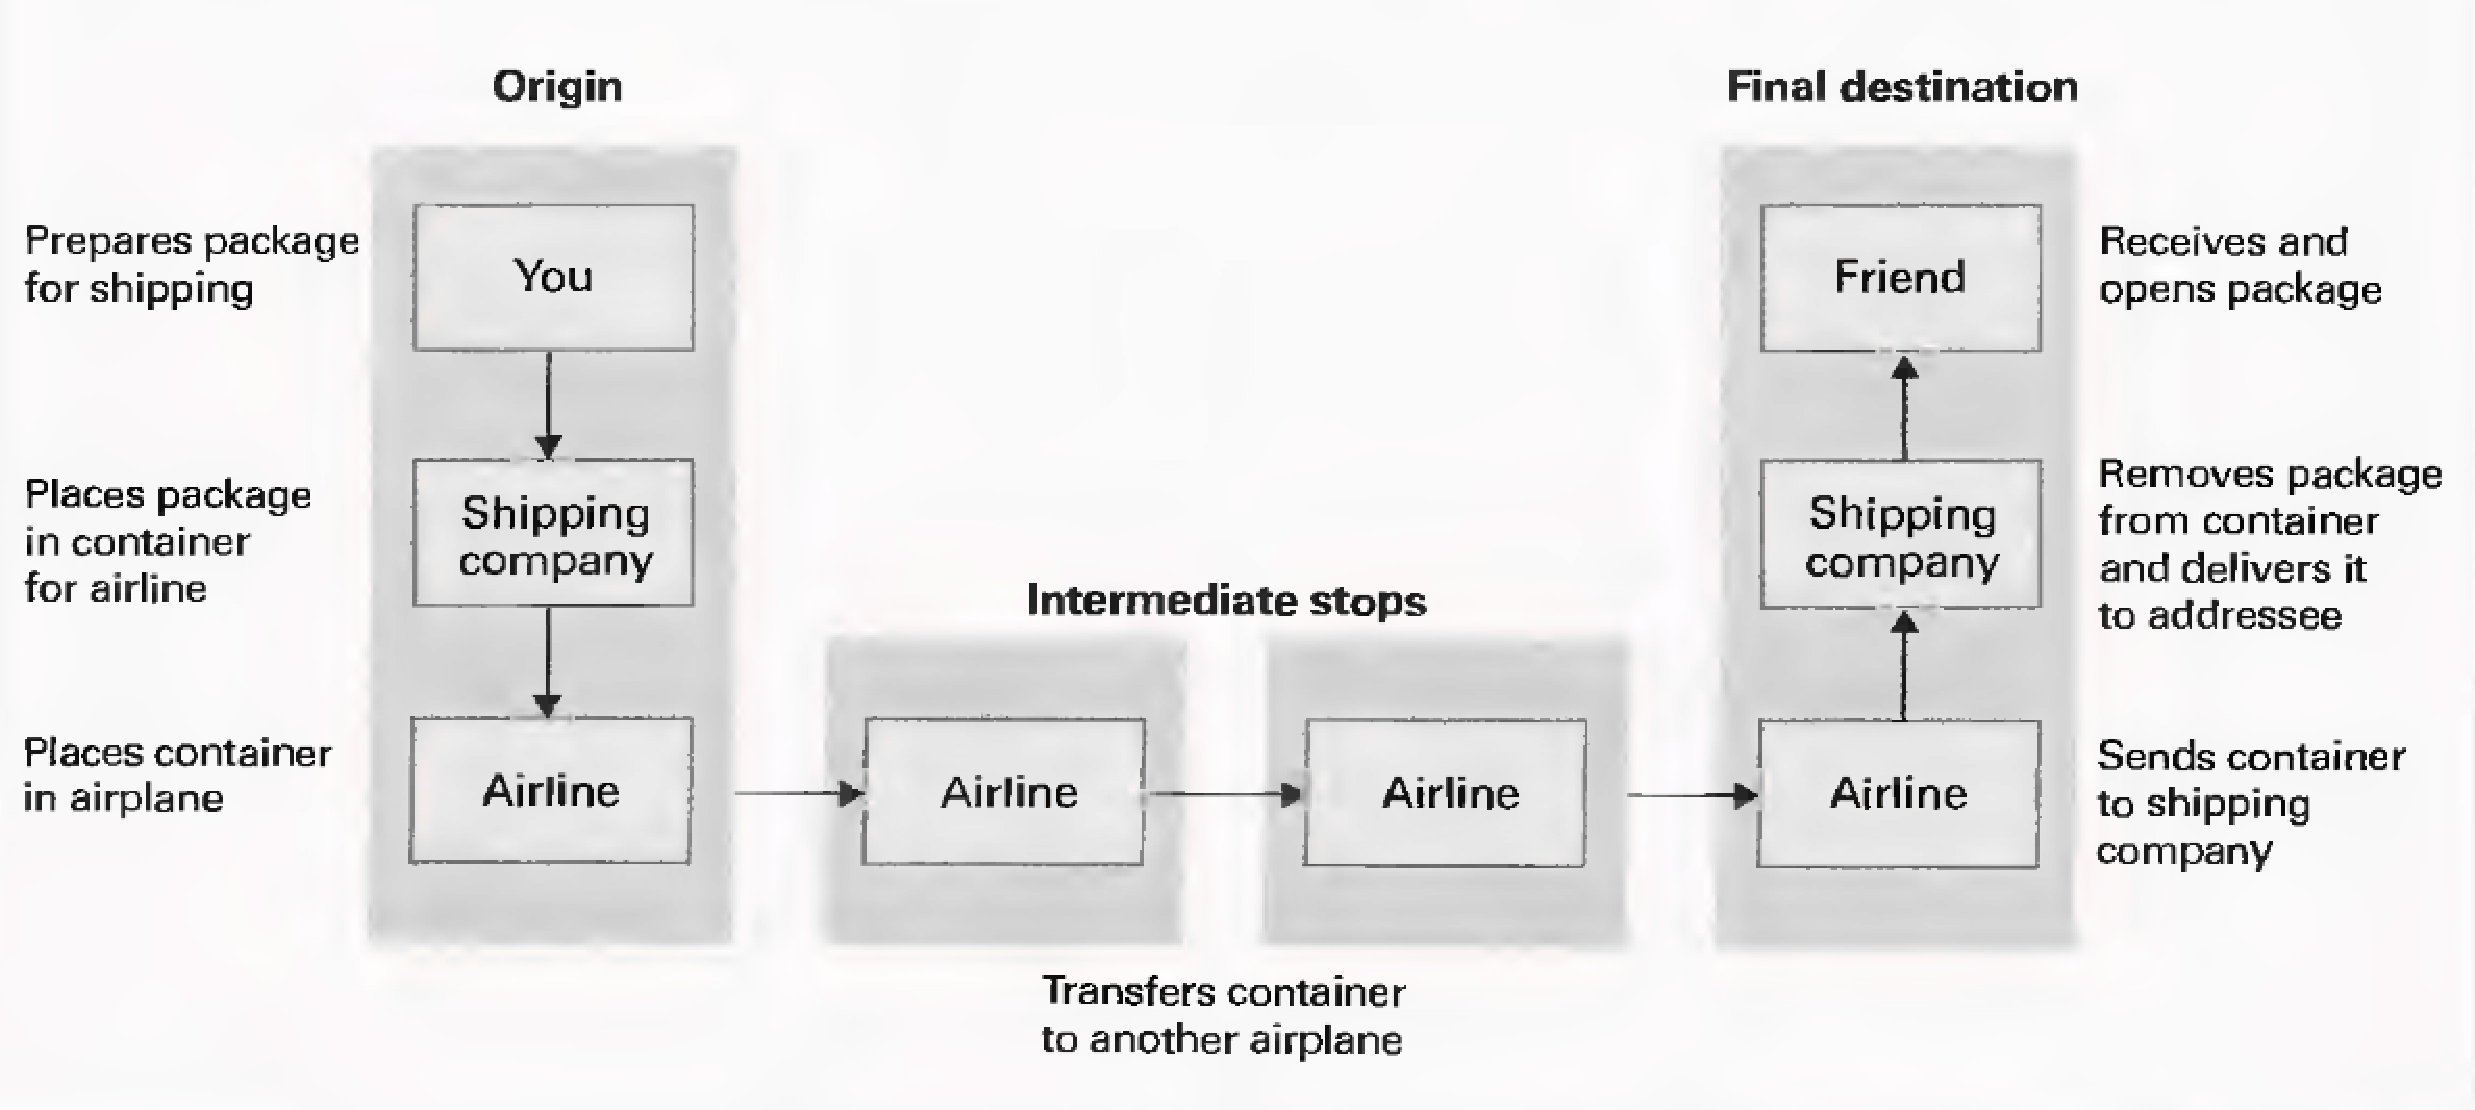
\includegraphics{ch5/fig412.pdf}}
  \caption{Ví dụ việc chuyển gói hàng hoá}
  \label{fig:fig4.12}
\end{figure}

Nói tóm lại, quá trình chuyên chở của gói hàng sẽ được thực hiện theo dạng cây ba cấp
(tầng):
\begin{inparaenum}[(a)]
\item cấp người sử dụng (bao gồm bạn và bạn bè của bạn),
\item công ty vận chuyển, và
\item hãng hàng không.
\end{inparaenum}
Mỗi cấp sử dụng cấp thấp hơn như là một công cụ trừu tượng. (Bạn không cần quan tâm tới
những chi tiết của công ty vận chuyển, và công ty vận chuyển cũng không cần quan tấm tới
những điều hành cục bộ của hãng hàng không.) Mỗi cấp độ trong cây ba cấp đều có những đại
diện ở cả nơi gửi và nơi nhận hàng,.

\begin{figure}[tbh]
  \centering \scalebox{0.35}{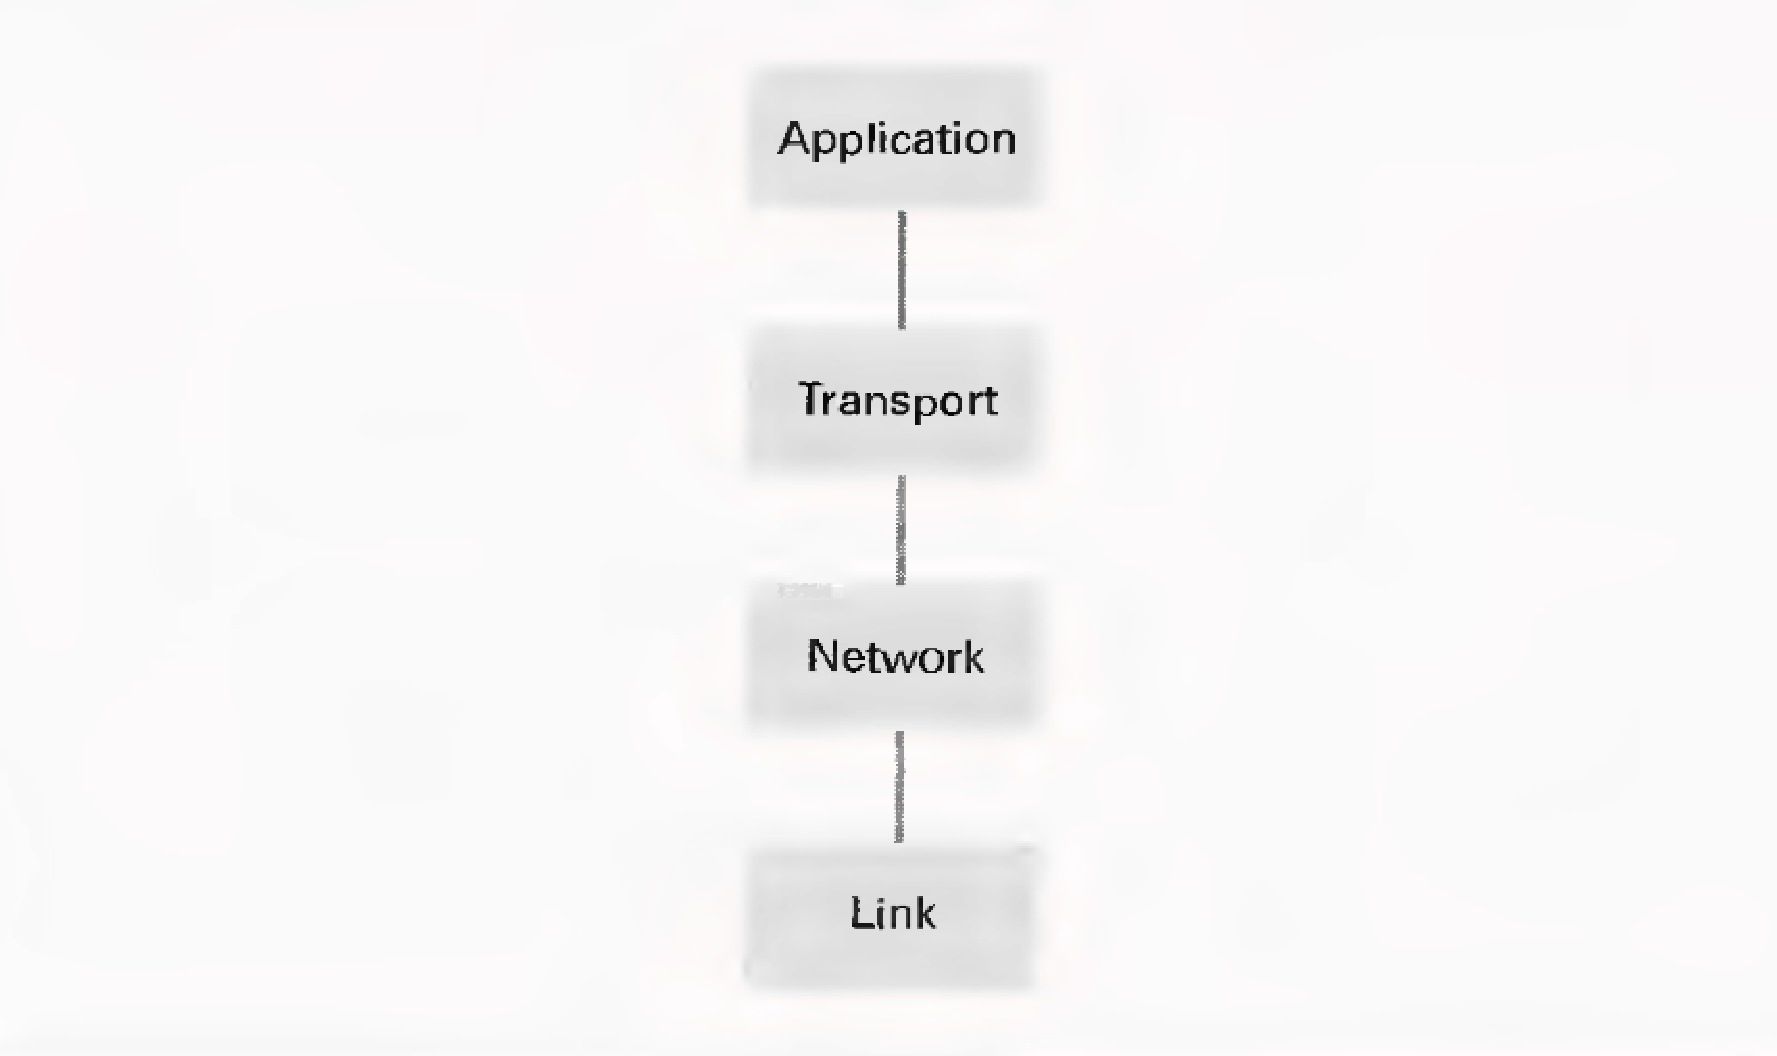
\includegraphics{ch5/fig413.pdf}}
  \caption{Các tầng phần mềm Internet}
  \label{fig:fig4.13}
\end{figure}

Ví dụ như trường hợp với sản phẩm điều khiển truyền thông qua mạng Internet, trừ phần mềm
Internet có bốn tầng chứ không phải ba tầng, thì mỗi phần mềm bao gồm một tập các chương
trình con đúng hơn là con người và công việc kinh doanh. Bốn tầng (cấp) này được biết đến
là \textbf{tầng ứng dụng}, \textbf{tầng vận chuyển}, \textbf{tầng mạng} và \textbf{tầng
  liên kết} (Hình~\ref{fig:fig4.13}). Tất cả các tầng đều hiện diện trên mỗi máy tính trên
mạng Internet. Một thông điệp thông thường đều bắt nguồn từ tầng ứng dụng. Từ đó nó được
chuyển qua xuống tầng vận chuyển và tầng mạng để chuẩn bị cho việc truyền tải, và cuối
cùng nó được truyền đi bởi tầng liên kết. Thông điệp đó được nhận bởi tầng liên kết phía
bên đích và được chuyển lên tầng trên cho đến khi nó được giao cho tầng ứng dụng tại đích
nhận của thông điệp.

Ta hãy xem xét quá trình này một cách kỹ lưỡng hơn bằng cách lần theo vết của một
thông điệp khi nó tìm đường qua hệ thống (Hình~\ref{fig:fig4.14}). Ta bắt đầu quá
trình lần vết tại tầng ứng dụng.


Tầng ứng dụng bao gồm các đơn vị phần mềm như phần mềm khách và phần mềm chủ mà sử dụng
truyền thông Internet để thực hiện những nhiệm vụ của chúng. Mặc dù tên của chúng là giống
nhau, tầng này không bị hạn chế các phần mềm theo sự phân loại ứng dụng được giới thiệu
trong Mục~\ref{sec:3.2}, nhưng cũng bao gồm nhiều gói tiện ích. Ví dụ, phần mềm truyền tải tệp sử
dụng giao thức truyền tệp (FTP) hay phần mềm cung cấp khả năng truy cập từ xa sử dụng
telnet trở nên phổ biến đến nỗi mà chúng thông thường được xem như là phần mềm tiện ích.


\begin{figure} 
  \centering \scalebox{0.5}{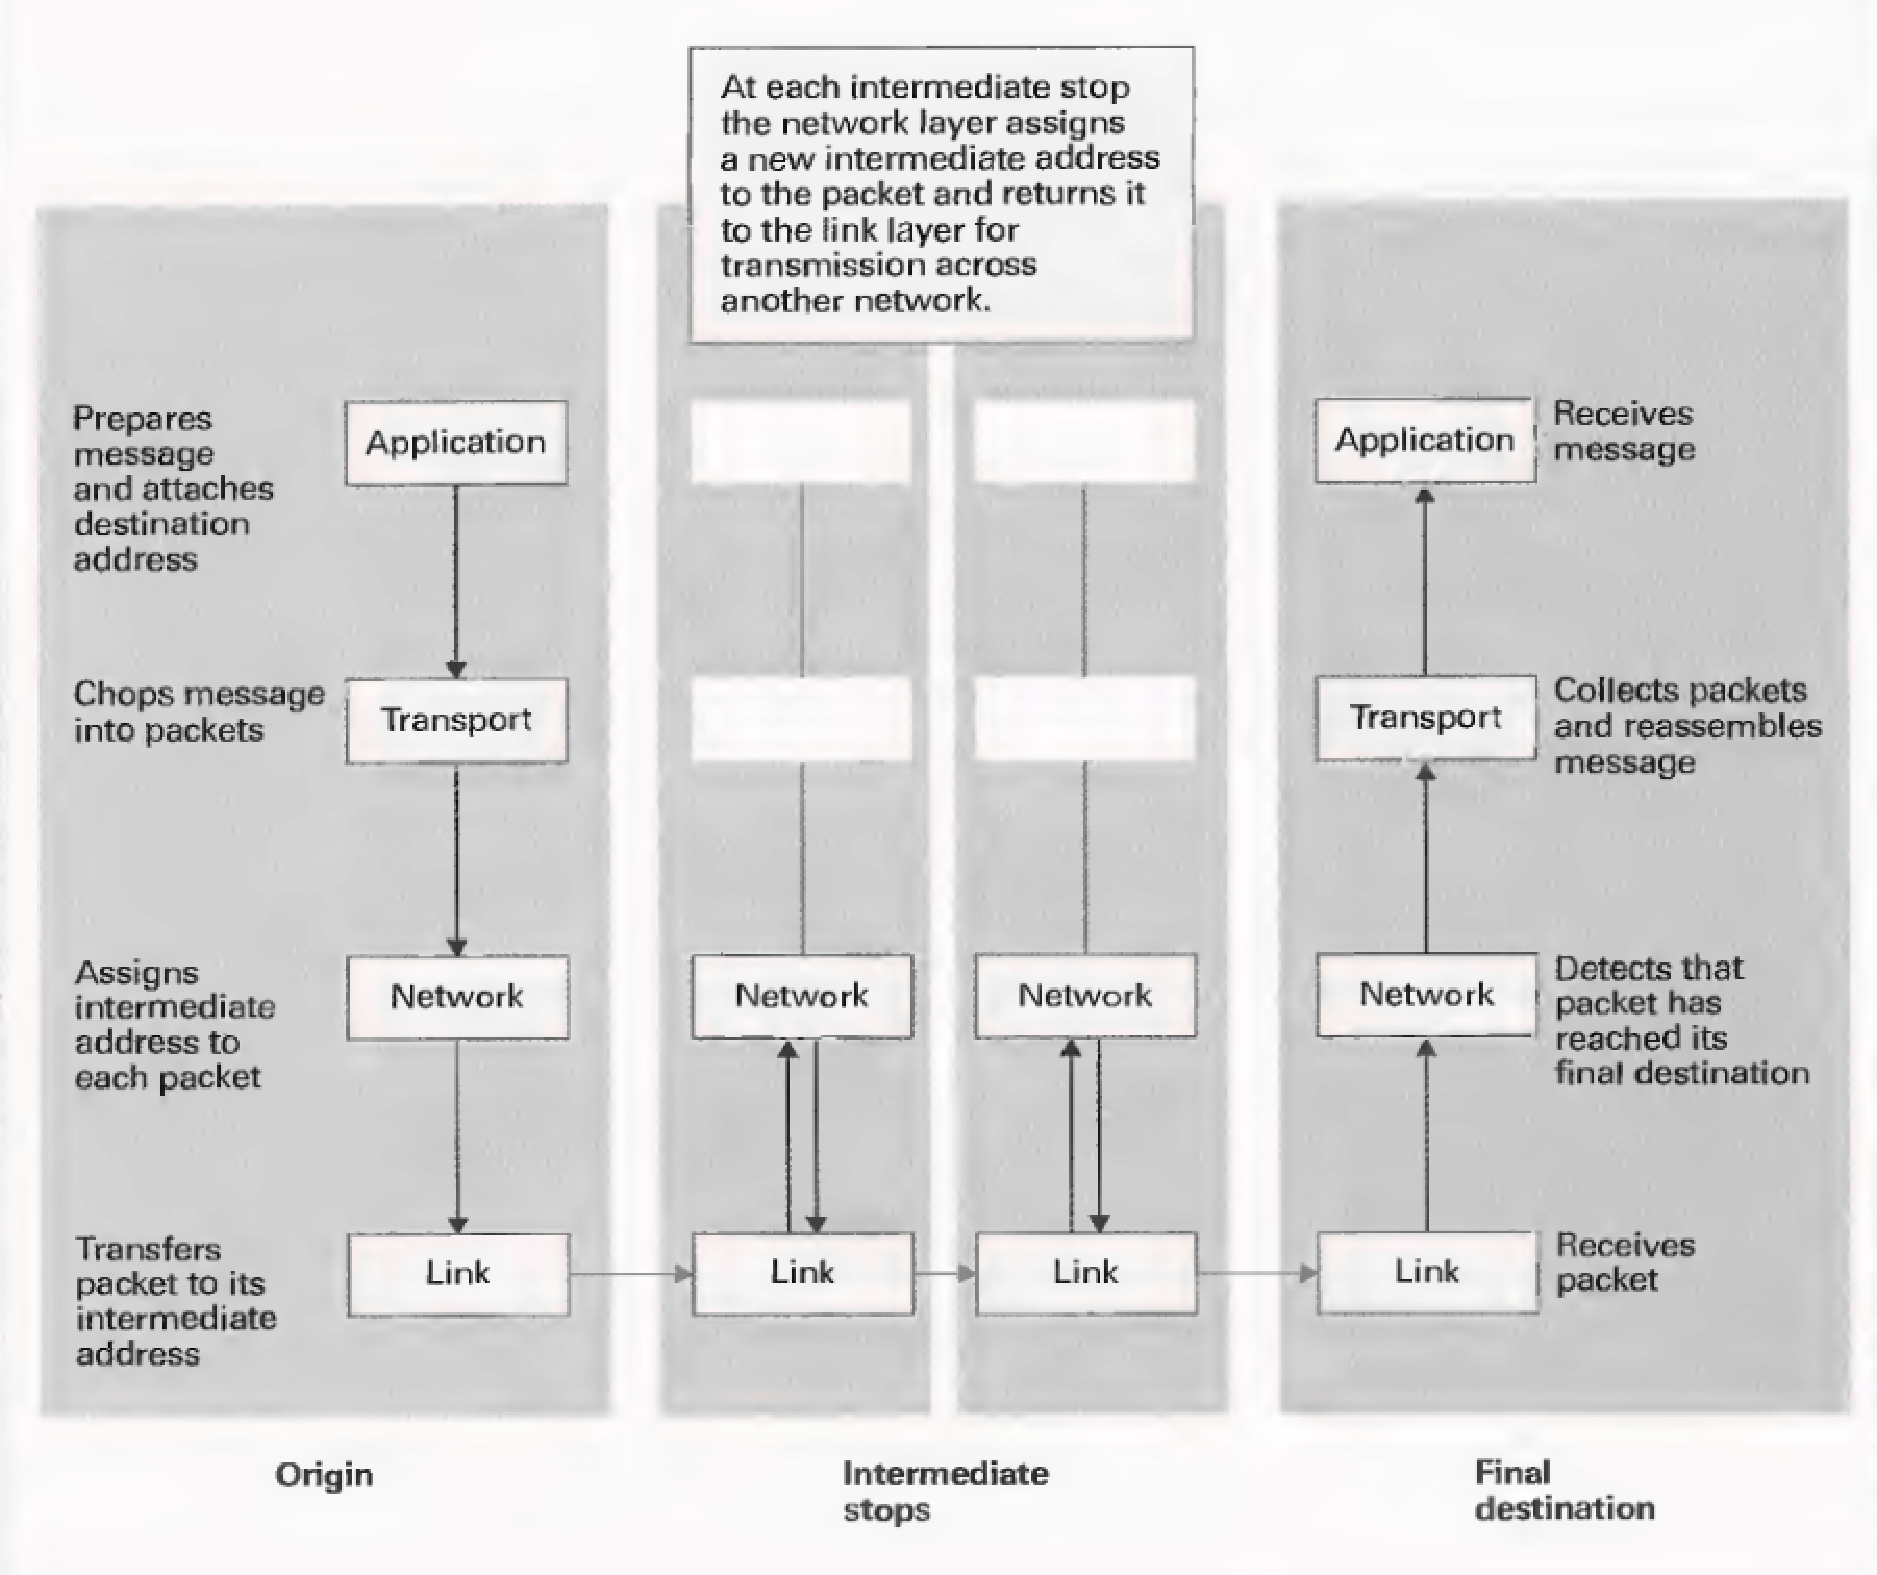
\includegraphics{ch5/fig414.pdf}}
  \caption{Truyền một thông điệp qua Internet}
  \label{fig:fig4.14}
\end{figure}


Tầng ứng dụng sử dụng tầng vận chuyển để gửi và nhận thông điệp qua Internet theo cùng một
cách thức mà ta sử dụng một công ty vận chuyển để gửi và nhận các gói hàng. Tương tự
như trách nhiệm của bạn là phải cung cấp một địa chỉ chi tiết hợp lệ với công ty vận
chuyển, trách nhiệm của tầng ứng dụng cũng là cung cấp một địa chỉ hợp lệ cho tầng vận
chuyển. (Để thực hiện được yêu cầu này, tầng ứng dụng có thể sử dụng các dịch vụ tên miền
trên Internet để chuyển đổi từ địa chỉ dễ nhớ được sử dụng bởi người dùng sang địa chỉ IP
tương thích với mạng Internet.)

Nhiệm vụ chính của tầng vận chuyển là chấp nhận các thông điệp đến từ tầng ứng dụng và đảm
bảo rằng những thông điệp này là đúng định dạng cho việc truyền tải qua mạng Internet. Để
phục vụ cho mục đích sau đó, tầng vận chuyển chia các thông điệp dài thành những đoạn nhỏ
(segment), mà sẽ được truyền qua mạng Internet như những đơn vị độc lập nhau. Việc chia
nhỏ này là cần thiết vì một thông điệp đơn và dài có thể làm tắc nghẽn luồng đi của những
thông điệp khác tại những điểm nút trên mạng Internet nơi mà rất nhiều thông điệp phải
được truyền qua những đoạn đường giao nhau.

Thật vậy, những đoạn thông điệp nhỏ có thể truyền xen lẫn với nhau tại những điểm nút thay vì một thông điệp dài bắt ép những thông điệp khác phải chờ trong khi nó truyền qua (giống
như những chiếc ô tô con phải chờ một đoàn tầu dài đi qua tại một ngã tư đường sắt).

Tầng vận chuyển thêm những số theo một trình tự vào những đoạn thông điệp nhỏ để các đoạn
này có thể được ghép nối lại tại đích của thông điệp. Sau đó nó gắn thêm địa chỉ đích vào
mỗi đoạn thông điệp và chuyển giao những đoạn thông điệp được đánh địa chỉ này, được biết
đến như là các gói tin (packet), cho tầng mạng. Từ đó, các gói tin được xử lý như những
thông điệp riêng rẽ và không liên quan đến nhau cho đến khi chúng được truyền tới tầng vận
chuyển tại đích cuối cùng của chúng.

Có thể nói là các gói tin gắn liền với một thông điệp chung có khả năng đi theo những
đường khác nhau qua mạng Internet.

Tầng mạng có nhiệm vụ là chuyển tiếp những gói tin nó nhận được từ một mạng trên Internet
tới một mạng khác trong quá trình chúng được chuyển tới đích cuối cùng của chúng. Theo
cách đó thì tầng mạng phải làm việc với mô hình của mạng Internet. Nói một cách cụ thể,
nếu đường đi của một gói tin qua mạng Internet phải được truyền qua rất nhiều mạng riêng
lẻ, nó chính là tầng mạng tại mỗi điểm dừng trung gian mà xác định hướng đi  gói tin sẽ
được gửi đi sau đó. Việt quyết định đưa ra ở đây là như sau: Nếu đích cuối cùng của gói
tin là thuộc bên trong của mạng hiện thời, tầng mạng sẽ gửi gói tin đến ngay đó; ngược
lại, tầng mạng sẽ gửi gói tin tới một thiết bị dẫn đường (router) trong mạng hiện tại,
thiết bị dẫn đường này sẽ có nhiệm vụ chuyển tiếp gói tin đến mạng gần kề. Theo cách thức
này thì một gói tin được gửi tới đích là một máy tính trong mạng hiện tại sẽ được gửi ngay
tới máy tính đó, ngược lại thì một gói tin được gửi tới một máy tính nằm ngoài mạng hiện
tại sẽ tiếp tục hành trình của nó từ mạng này sang mạng tiếp theo gần kề cho đến mạng đích
cuối cùng.

Để quyết định đích tiếp theo trong hành trình của gói tin, tầng mạng cập nhật thêm địa chỉ
này vào gói tin như là một địa chỉ trung gian và chuyển giao gói tin này xuống tầng liên
kết.

Tầng liên kết có trách nhiệm truyền tải gói tin tới địa chỉ trung gian mà đã được xác định
bởi tầng mạng ở trên. Do đó, tầng liên kết phải thỏa thuận với sự truyền thông tới mạng
riêng biệt của máy tính. Nếu mạng đó là mạng vòng tròn có sử dụng thẻ bài, tầng liên kết
phải đợi có quyền chiếm hữu thẻ bài trước khi truyền gói tin đi. Nếu mạng sử dụng CSMA/CD,
tầng liên kết phải lắng nghe khi đường trục truyền rỗi mới được thực hiện truyền tải.

Khi một gói tin được truyền đi, nó được nhận bởi tầng liên kết tại máy tính được chỉ định
rõ bởi địa chỉ cục bộ đã được gắn thêm vào thông điệp. Tại đó, tầng liên kết sẽ chuyển
giao gói tin lên tầng mạng, nơi mà đích cuối cùng của gói tin được so sánh và kiểm tra với
địa chỉ hiện tại. Nếu những địa chỉ này không trùng khớp, tầng mạng xác định một địa chỉ
trung gian mới cho gói tin, đính kèm địa chỉ đó vào gói tin và đưa gói tin quay trở về
tầng liên kết để tiếp tục thực hiện truyền gói tin đi. Trong cách thức này, mỗi gói tin
được chuyển qua từng máy tính trên hành trình tới đích của nó. Cần chú ý rằng chỉ có tầng
liên kết và tầng mạng mới liên quan tại những điểm dừng trung gian trong suốt hành trình
này (xem lại Hình~\ref{fig:fig4.14}).

Nếu tầng mạng xác định rằng một gói tin đến đã tiến tới được đích cuối cùng, nó sẽ chuyển
giao gói tin đó cho tầng vận chuyển. Khi tầng vận chuyển nhận được các gói tin được gửi
tới từ tầng mạng, nó sẽ bóc tách những thông tin cần thiết bên trong của những đoạn tin và
xây dựng lại thông điệp gốc ban đầu dựa trên những số trình tự mà đã được cung cấp bởi
tầng vận chuyển tại nơi gửi của thông điệp. Khi thông điệp được ghép nối lại, tầng vận
chuyển thực hiện chuyển giao nó cho đơn vị phần mềm thích hợp trên tầng ứng dụng--kết thúc
quá trình truyền thông của thông điệp.


Việc xác định xem đơn vị phần mềm nào trong tầng ứng dụng được phép nhận một thông điệp
được gửi tới là nhiệm vụ quan trọng của tầng vận chuyển. Nhiệm vụ này được thực hiện thông
qua việc gán những \textbf{số cổng} duy nhất (không liên quan đến những cổng I/O đã được
thảo luận trong Chương~\ref{chap:2}) cho các đơn vị phần mềm khác nhau và yêu cầu số cổng thích
hợp được chèn thêm vào địa chỉ của thông điệp trước khi bắt đầu gửi thông điệp. Sau đó,
khi thông điệp được nhận bởi tầng vận chuyển tại đích nhận, tầng vận chuyển chỉ đơn thuần
chuyển giao thông điệp đó cho phần mềm trên tầng ứng dụng có cổng được chỉ định trước.

Người sử dụng của mạng Internet rất hiếm khi cần phải quan tâm tới những con số cổng này
bởi vì những ứng dụng thông thường thường có những cổng đã được công nhận một cách phổ
biến. Ví dụ, nếu một trình duyệt Web được yêu cầu tải một tài liệu mà URL của nó là
\url{http://www.zoo.org/animals/frog.html}, trình duyệt sẽ thừa nhận rằng nó cần phải liên
lạc với một phần mềm chủ HTTP tại địa chỉ \url{www.zoo.org} thông qua cổng 80. Tương tự
như vậy, khi truyền tải một tệp, một phần mềm khách FTP cũng thừa nhận rằng nó cần phải
giao tiếp với phần mềm chủ FTP thông qua cổng~20 và 21.

Nói tóm lại, việc truyền thông qua mạng Internet bao gồm sự tương tác giữa bốn tầng của
phần mềm. Tầng ứng dụng xử lý các thông điệp đứng trên góc độ tầm nhìn của ứng dụng. Tầng
vận chuyển chuyển đổi những thông điệp này thành những gói tin mà tương thích với mạng
Internet và tập hợp những thông điệp mà nhận được trước khi giao chúng cho ứng dụng thích
hợp. Tầng mạng liên quan đến việc gửi trực tiếp những gói tin qua mạng Internet. Tầng liên
kết đảm nhận việc truyền thông thực sự của những gói tin từ máy tính này tới máy tính
khác. Với tất cả các hoạt động này, có thể nói là hết sức kinh ngạc với thời gian trả lời
của mạng Internet được đo lường theo đơn vị phần nghìn giây (millisecond) thì rất nhiều
giao dịch xuất hiện ngay tức thời.

\subsection*{Bộ giao thức TCP/IP}

Yêu cầu đặt ra cho các hệ thống mạng mở đã phát sinh một nhu cầu cho những chuẩn được
công bố bởi các hãng sản xuất có thể cung cấp thiết bị và phần mềm mà hoạt động một cách
đúng đắn với những sản phẩm của các hãng khác. Một chuẩn mà kết quả là mô hình tham chiếu
Hệ thống mở kết nối liên mạng (OSI: Open System Interconnection), đã được đưa ra bởi Tổ
chức quốc tế về tiêu chuẩn hóa (International Organization Standardization). Chuẩn này
được dựa trên một hệ thống phân cấp bảy tầng trái với hệ thống phân cấp bốn tầng mà chúng
ta đã xem xét ở trên. Nó là một mô hình often-quoted vì nó mang theo uy quyền của một tổ
chức quốc tế, nhưng nó cũng làm trì hoãn việc thay thế quan điểm về mô hình bốn tầng, chủ
yếu là bởi vì nó được thiết lập sau hệ thống phân cấp bốn tầng vốn đã trở thành một chuẩn
trên thực tế cho mạng Internet.


Bộ giao thức TCP/IP là một tập các giao thức được sử dụng bởi mạng Internet nhằm triển
khai việc liên lạc theo hệ thống phân cấp trên mạng Internet. Trên thực tế, \textbf{Giao
  thức Điều khiển Việc truyền tải(TCP)} (TCP: Transmission Control Protocol) và
\textbf{Giao thức Mạng Internet (IP)} (IP: Internet Protocol) là tên của chỉ hai trong số
những giao thức trong tập giao thức rộng lớn này--thực tế là toàn bộ tập hợp này được hiểu
như là bộ giao thức TCP/IP. Một cách chính xác hơn, TCP định nghĩa một phiên bản của tầng
vận chuyển. Ta phát biểu là một phiên bản bởi vì bộ giao thức TCP/IP cung cấp hơn
một cách thức thực thi tại tầng vận chuyển; một phiên bản khác được định nghĩa bởi giao
thức UDP (User Datagram Protocol). Việc tách đôi như vậy cũng tương tự như trên thực tế
khi việc vận chuyển một gói hàng, bạn có một lựa chọn giữa nhiều công ty vận chuyển, mỗi
công ty lại đưa ra dịch vụ cơ bản là giống nhau nhưng cũng vẫn có những nét đặc trưng duy
nhất cho từng công ty. Do phụ thuộc vào chất lượng đặc biệt của dịch vụ đã yêu cầu, một
đơn vị trên tầng ứng dụng có thể lựa chọn gửi dữ liệu đi thông qua một trong hai phiên bản
của tầng vận chuyển, TCP hoặc UDP (Hình~\ref{fig:fig4.15})

\begin{figure} [tbh]
  \centering \scalebox{0.5}{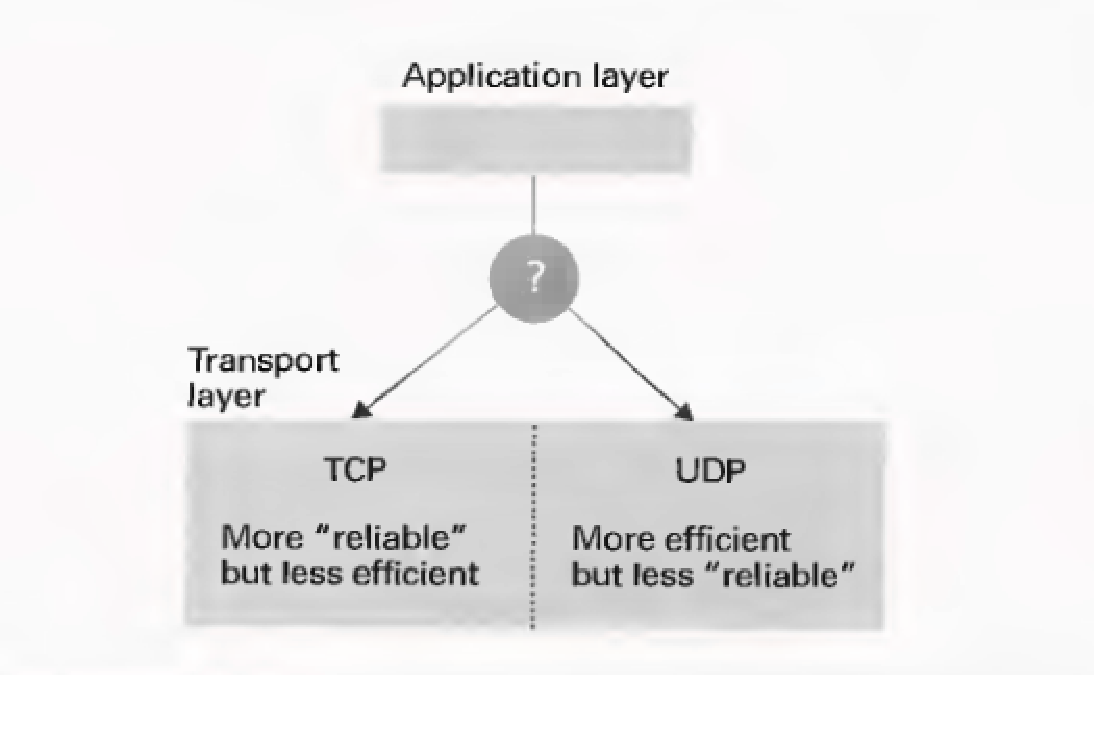
\includegraphics{ch5/fig415.pdf}}
  \caption{Lựa chọn giữa TCP và UDP}
  \label{fig:fig4.15}
\end{figure}


Có hai điểm khác biệt cơ bản giữa TCP và UDP. Thứ nhất là trước khi gửi một thông điệp
được yêu cầu bởi tầng ứng dụng, tầng vận chuyển sử dụng giao thức TCP để gửi thông điệp
của chính nó tới tầng vận chuyển của bên đích nói rằng một thông điệp sắp được gửi sang
đó. Sau đó nó sẽ chờ thông điệp này được công nhận trước khi bắt đầu gửi thông điệp của
tầng ứng dụng. Theo cách đó, tầng vận chuyển sử dụng giao thức TCP sẽ thiết lập một kết
nối trước khi gửi một thông điệp. Còn tầng vận chuyển sử dụng giao thức UDP không thiết
lập một kết nối như vậy trước khi gửi một thông điệp. Tầng vận chuyển chỉ đơn thuần gửi
thông điệp nào đó tới địa chỉ mà nó nhận được và không quan tâm đến địa chỉ đó. Với tất cả
những gì mà nó biết được, máy tính đích có thể không sẵn sàng hoạt động. Với lý do này,
UDP được gọi là giao thức không có kết nối.

Sự khác biệt cơ bản thứ hai giữa TCP và UDP là tầng vận chuyển sử dụng giao thức TCP tại
nguồn gửi và đích nhận là cùng làm việc với nhau theo cách thức trả lời xác nhận và truyền
lại gói tin nhằm chắc chắn rằng tất cả các đoạn tin của thông điệp thực sự đã được truyền
tới đích thành công. TCP được gọi là giao thức tin cậy, trong khi đó thì UDP do không đưa
ra dịch vụ truyền lại nên được gọi là giao thức không tin cậy. Điều này không có nghĩa là
UDP là một lựa chọn tồi. Sau tất cả những điều trên, ta có thể kết luận tầng vận
chuyển sử dụng giao thức UDP được tổ chức hợp lý hơn so với tầng vận chuyển sử dụng giao
thức TCP, và do đó nếu một ứng dụng được chuẩn bị để có thể đạt được những kết quả tiềm
tàng của UDP, ý kiến đó có thể sẽ là một sự lựa chọn tốt hơn. Ví dụ, thư điện tử (email)
thông thường được gửi thông qua giao thức TCP nhưng sự truyền tải thực hiện thông qua hệ
thống máy chủ tên miền khi chuyển đổi những địa chỉ từ dạng dễ nhớ sang dạng IP lại sử
dụng giao thức UDP.

IP là một chuẩn của mạng Internet đối với tầng mạng. Một trong số những đặc tính của nó là
mỗi khoảng thời gian tầng mạng sử dụng giao thức IP lại chuẩn bị một gói tin để gửi xuống
tầng liên kết, nó sẽ thêm một giá trị được gọi là bộ đếm bước truyền, hay thời gian sống
(time to live), vào gói tin đó. Giá trị này là một giới hạn cho số lần gói tin được chuyển
tiếp khi nó cố thử tìm một đường đi qua mạng Internet. Mỗi khoảng thời gian tầng mạng sử
dụng giao thức IP chuyển tiếp một gói tin, nó sẽ giảm bộ đếm bước truyền xuống một giá
trị. Với thông tin này, tầng mạng có thể bảo vệ cho mạng Internet bởi sự lặp vòng vô hạn
của các gói tin trong hệ thống. Cho dù mạng Internet vẫn tiếp tục phát triển từ những thời
sơ khai của nó, một bộ đếm bước truyền ban đầu với giá trị là 64 là chưa đủ để cho phép
một gói tin có thể tìm được đường đi của nó khi được truyền xuyên suốt qua mê cung của
những mạng LAN, MAN, WAN, và các bộ dẫn đường.

Cho đến nay một phiên bản của giao thức IP được biết đến là IPv4 (IP phiên bản 4) đã được
sử dụng trong việc thực thi tầng mạng trong mạng Internet. Tuy nhiên, mạng Internet đã
nhanh chóng phát triển và vượt ra ngoài phạm vi hệ thống 32 bít địa chỉ của IPv4. Do đó,
một phiên bản mới của giao thức IP được biết đến là Ipv6, sử dụng địa chỉ liên mạng bao
gồm 128 bít, đã được thiết lập. Quá trình chuyển đổi từ IPv4 sang IPv6 hiện nay vẫn đang
thực hiện. (Đây là sự chuyển đổi mà ta đã được xem xét qua phần giới thiệu về địa
chỉ Internet trong Mục~\ref{sec:4.2}) Trong một vài phạm vi, IPv6 đang được sử dụng trên thực tế;
một vài phạm vi khác, sự chuyển đổi vẫn đang tiếp diễn trong một vài năm nữa. Ví dụ, theo
những kế hoạch hiện tại của chính phủ Hoa Kỳ là chuyển đổi sang IPv6 trước năm 2008. Trong
bất kỳ trường hợp nào, địa chỉ 32 bít trên mạng Internet vẫn được mong đợi là sẽ không còn
được sử dụng trước năm 2025.

\subsection*{Câu hỏi \& Bài tập}

\begin{enumerate}
\item Những tầng nào trong hệ thống phân cấp của phần mềm Internet được sử dụng để chuyển
  tiếp một thông điệp đến sang một máy tính khác?

\item Chỉ ra một vài sự khác biệt giữa tầng vận chuyển sử dụng giao thức TCP và tầng vận
  chuyển sử dụng giao thức UDP?

\item Làm thế nào để phần mềm Internet có thể đảm bảo rằng các thông điệp không bị chuyển
  tiếp trên mạng Internet mãi mãi?

\item Điều gì khiến cho một máy tính trên mạng Internet tránh được thao tác ghi lại các
  bản sao của những thông điệp truyền qua nó?

\end{enumerate}


%%% Local Variables: 
%%% mode: latex
%%% TeX-master: "../tindaicuong"
%%% End: 
